\documentclass{article}

\title{Econ815: Problem Set 7}
\date{December 4, 2017}
\author{Matthew Harvey}
\usepackage{amsmath}
\usepackage{graphicx}

\begin{document}
\maketitle

\section*{The Stationary Distribution}
Having moved through calculations with the given parameters, we arrive at the following distribution of firms in the general equilibrium. Below I graph the result of this from my code.

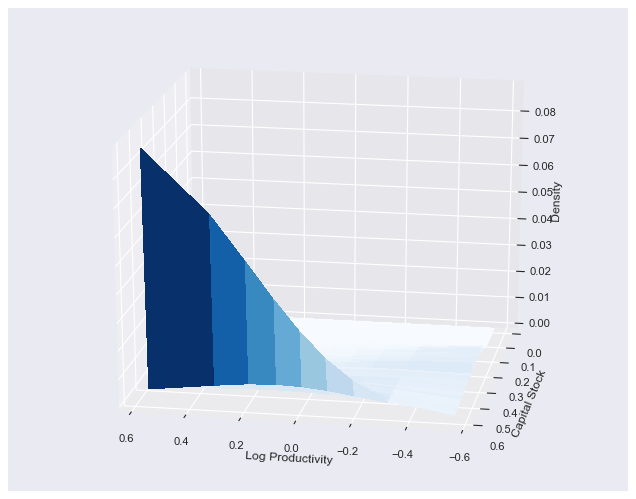
\includegraphics[width=75mm,scale=0.1]{panic_station.png}

This graphs the equilibrium distribution of firms for shock levels and amount of capital. Higher shocks are associated with more firms in the market as are higher levels of capital. This fits with classical theory since rising firm profits (as would likely be the case here) would cause more firms to enter.

\section*{Wage Rate}
Here the optimal wage rate is $1.06215292$

\section*{The Policy Function}
Below I plot the policy function for each specific firm. Here is it worth noting that rising productivity leads to a greater level of optimal capital.

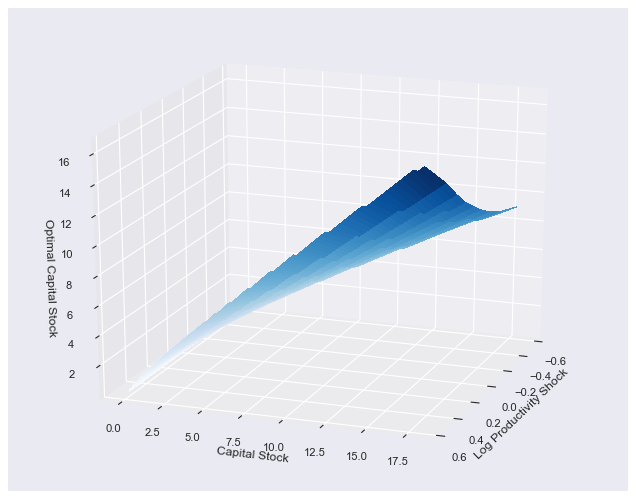
\includegraphics[width=75mm,scale=0.1]{policy.png}

In the three dimensional graph, the optimal capital stock peaks out at the highest level of productivity. Thus, as one attains higher productivity shocks, it becomes optimal to have more capital.

\section*{Reflections}
My initial coding attempts failed to yield a solution in any reasonable amount of time (each iteration took nearly a minute to run) due to the modularization of the code. I have placed the modules in the folder along with the actual result. Putting all the code in a single file created a script that ran iteration is eighty times less time.

\end{document}